\documentclass[12pt]{report}
\usepackage[utf8]{inputenc}
\usepackage[russian]{babel}
%\usepackage[14pt]{extsizes}
\usepackage{listings}

% Для листинга кода:
\lstset{ %
language=python,                 % выбор языка для подсветки (здесь это С)
basicstyle=\small\sffamily, % размер и начертание шрифта для подсветки кода
numbers=left,               % где поставить нумерацию строк (слева\справа)
numberstyle=\tiny,           % размер шрифта для номеров строк
stepnumber=1,                   % размер шага между двумя номерами строк
numbersep=5pt,                % как далеко отстоят номера строк от подсвечиваемого кода
showspaces=false,            % показывать или нет пробелы специальными отступами
showstringspaces=false,      % показывать или нет пробелы в строках
showtabs=false,             % показывать или нет табуляцию в строках
frame=single,              % рисовать рамку вокруг кода
tabsize=2,                 % размер табуляции по умолчанию равен 2 пробелам
captionpos=t,              % позиция заголовка вверху [t] или внизу [b] 
breaklines=true,           % автоматически переносить строки (да\нет)
breakatwhitespace=false, % переносить строки только если есть пробел
escapeinside={\#*}{*)}   % если нужно добавить комментарии в коде
}

% Для измененных титулов глав:
\usepackage{titlesec, blindtext, color} % подключаем нужные пакеты
\definecolor{gray75}{gray}{0.75} % определяем цвет
\newcommand{\hsp}{\hspace{20pt}} % длина линии в 20pt
% titleformat определяет стиль
\titleformat{\chapter}[hang]{\Huge\bfseries}{\thechapter\hsp\textcolor{gray75}{|}\hsp}{0pt}{\Huge\bfseries}


% plot
\usepackage{pgfplots}
\usepackage{filecontents}
\usetikzlibrary{datavisualization}
\usetikzlibrary{datavisualization.formats.functions}

\begin{document}
 
%\def\chaptername{} % убирает "Глава"
\begin{titlepage}
	\centering
	{\scshape\LARGE МГТУ им. Баумана \par}
	\vspace{3cm}
	{\scshape\Large Лабораторная работа №7\par}
	\vspace{0.5cm}	
	{\scshape\Large По курсу: "Анализ алгоритмов"\par}
	\vspace{1.5cm}
	{\huge\bfseries Поиск в словаре \par}
	\vspace{2cm}
	\Large Работу выполнил: студент группы ИУ7-53Б Наместник Анастасия\par
	\vspace{0.5cm}
	\LargeПреподаватели:  Волкова Л.Л., Строганов Ю.В.\par

	\vfill
	\large \textit {Москва, 2020} \par
\end{titlepage}

\tableofcontents

\newpage
\chapter*{Введение}
\addcontentsline{toc}{chapter}{Введение}

В жизни широко распространены словари, например, привычные бумажные словари (толковые, орфографические, лингвистические). В них ключом является слово-заголовок статьи, а значением — сама статья. Для того, чтобы получить доступ к статье, необходимо указать слово-ключ. В программировании принцип устройства словаря тот же самый. В этой лабораторной буду рассмотрены алгоритмы поиска значения по ключу в словаре. 
	
Целью данной лабораторной работы является изучение поиска значения по ключу в словаре с помощью алгоритмов поиска полным перебором, двоичного поиска в упорядоченном словаре и частичного анализа.

В данной лабораторной работе требуется решить пять задач:
\begin{itemize}
\item изучить алгоритм поиска в словаре полным перебором;
\item изучить алгоритм двоичного поиска в упорядоченном словаре;
\item изучить алгоритм частичного анализа для поиска в словаре;
\item программно реализовать описанные выше алгоритмы;
\item провести сравнительный анализ скорости работы реализованных алгоритмов.
\end{itemize}


\chapter{Аналитическая часть}

В этом разделе будут представлены теоретические сведения, необходимые для программной реализации поиска значения в словаре по ключу.
 
\section{Понятие словаря}
 \textbf{Словарь} - это ассоциативный массив, позволяющий хранить пары вида «(ключ, значение)» и поддерживающий операции добавления пары, а также поиска и удаления пары по ключу. Предполагается, что ассоциативный массив не может хранить две пары с одинаковыми ключами. В паре (k, v) значение v называется значением, ассоциированным с ключом k. Где k - это key, а v - это value.  Семантика и названия вышеупомянутых операций в разных реализациях ассоциативного массива могут отличаться\cite{AssocArray}.
Ассоциативный массив с точки зрения интерфейса удобно рассматривать как обычный массив, в котором в качестве индексов можно использовать не только целые числа, но и значения других типов — например, строки.
Поддержка ассоциативных массивов есть во многих интерпретируемых языках программирования высокого уровня, таких, как Perl\cite{Perl}, PHP\cite{Php}, Python\cite{Python}, Ruby\cite{Ruby}, JavaScript\cite{JS} и других.
Существует несколько вариантов поиска значения в словаре по ключу. Будут рассмотрены три из них:
\begin{itemize}
\item поиск в словаре полным перебором;
\item двоичный поиск в упорядоченном словаре;
\item частичный анализ для поиска в словаре.
\end{itemize}

\section{Поиск полным перебором}
Поиск \textit{полным перебором} подразумевает последовательный проход по словарю со сравнением ключа искомого значения с i-ым ключом словаря на i-ом шаге цикла. Возможно (N + 1) случаев: ключ не найден и N возможных случаев расположения ключа в словаре. Лучший случай: за одно сравнение ключ найден в начале словаря. Худших случаев 2: за N сравнений либо элемент не найден, либо ключ найден на последнем сравнении. Пусть на старте алгоритм поиска затрагивает k0 операций, а при каждом сравнении k1 (2 константы). Тогда в лучшем случае будет затрачено k0 + k1 операций. В случае, если ключ будет найден на 2ой позиции, будет затрачено k0 + 2 * k1 операций, на последней позиции - k0 + N * k1 операций, столько же, если ключ не будет найден вовсе. 	

\section{Двоичный поиск в упорядоченном словаре}
Если исходный массив уже отсортирован, то элемент в нем можно найти гораздо быстрее, если воспользоваться идеей \textit{двоичного (бинарного) поиска}. Идея заключается в делении списка пополам, после чего в зависимости от значения медианного элемента в списке мы переходим либо к левой, либо к правой половине списка. Тем самым, длина части, в которой мы ищем элемент, сокращается в два раза на каждом шаге цикла, а, значит, общая сложность алгоритма двоичного поиска будет O(log_{2}n).

 На рис. 2.1 представлен пример решения задачи поиска элемента в массиве бинарным поиском.

\begin{center}
		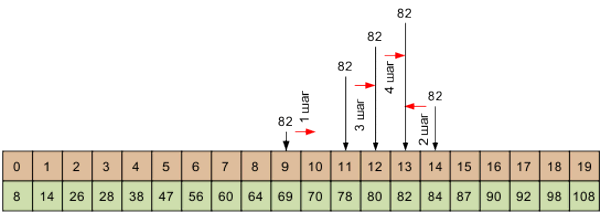
\includegraphics[scale=1.9]{pics/BinSearch.png}
		
			Рис 2.1: Двоичный (бинарный) поиск
\end{center}

\section{Частичный анализ}
\textit{Частичный анализ} подразумевает, что словарь отсортирован по частоте встречаемости первого символа каждого ключа словаря. Ключами k нового словаря, сформированного на основе исходного, являются буквы алфавита, с которыми ассоциированы значения - словари, первая буква ключей которых совпадает с ключами k основного словаря. Такая организация напоминает толковый словарь. Изначально поиск осуществляется по первой букве ключа искомого значения, затем в найденном словаре поиск продолжается полным перебором. 

\section{Используемые данные}
В этой лабораторной работе были использованы данные, представляющие таблицу пациентов, инфицированных COVID-19, в период от 01.01.2020 до 22.02.2020. Ключом является имя пациента, а значение - это структура со следующими полями:
\begin{itemize}
\item reporting\_date - дата регистарции пациента;
\item gender - пол;
\item age -возраст;
\item symptom\_onset - дата начала проявления симптомов;
\item hosp\_visit\_date - дата посещения больницы;
\item id\_status - статус состояния здоровья.
\end{itemize} 

\section{Вывод}

В данном разделе были рассмотрены теоретические сведения, необходимые для программной реализации поиска значения в словаре по ключу.
 
\chapter{Конструкторская часть}

В данном разделе будут представлены схемы реализации алгоритма полного перебора, алгоритма двоичного поиска и алгоритма частичного анализа.

Схема реализации алгоритма полного перебора представлена на рис. 2.2.

\begin{center}
		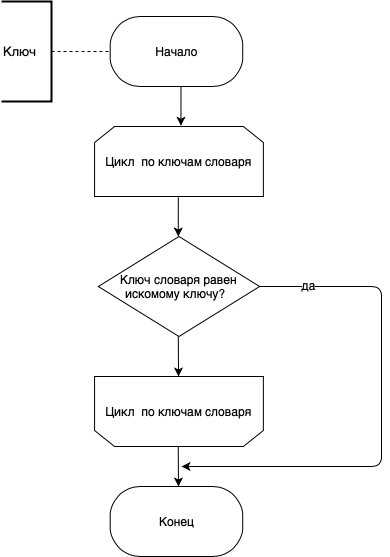
\includegraphics[scale=0.6]{schema/Brute.png}
		
			Рис 2.2: Схема реализации алгоритма полного перебора
\end{center}

Схема реализации алгоритма двоичного поиска представлена на рис. 2.3.

\begin{center}
		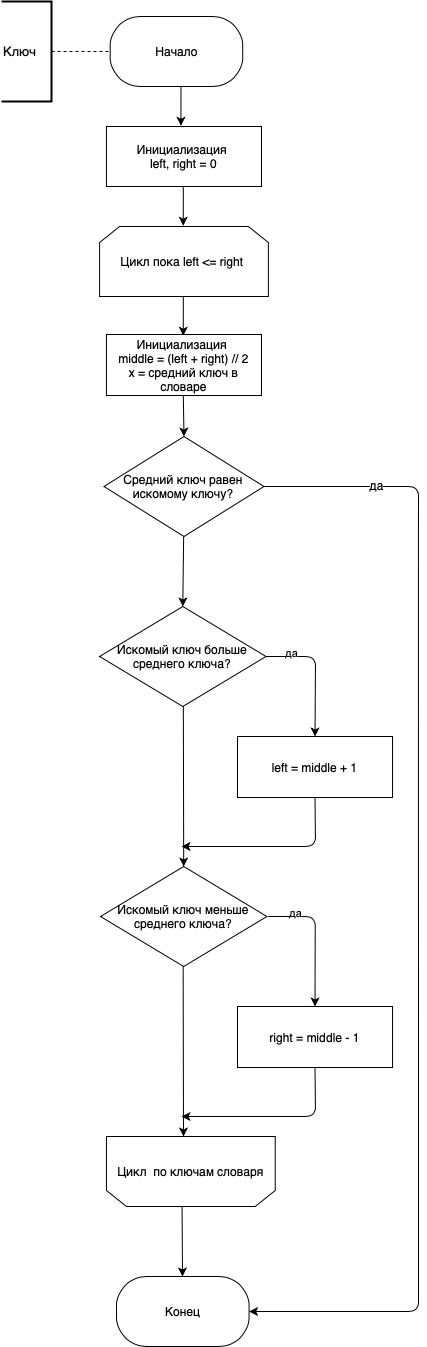
\includegraphics[scale=0.4]{schema/Bin.png}
		
			Рис 2.3: Схема реализации алгоритма двоичного поиска
\end{center}

Схема реализации алгоритма частичного анализа представлена на рис. 2.4.

\begin{center}
		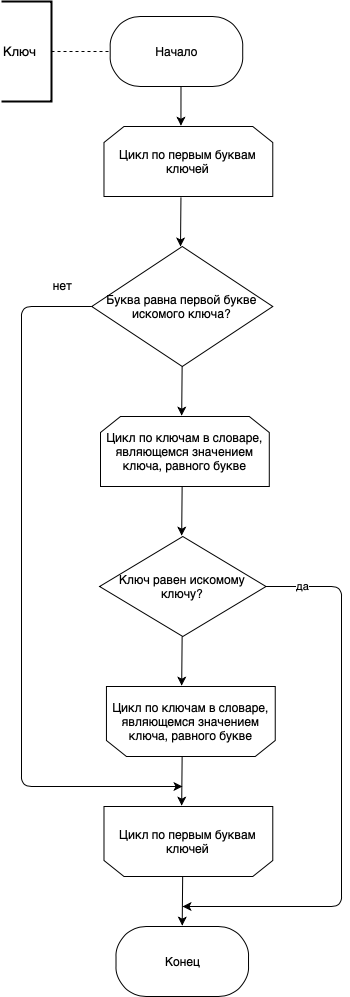
\includegraphics[scale=0.5]{schema/PartAnalysis.png}
		
			Рис 2.4: Схема реализации алгоритма частичного анализа
\end{center}


\section{Вывод}
В данном разделе были рассмотрены 3 схемы: схема реализации алгоритма полного перебора, схема алгоритма двоичного поиска и схема алгоритма частичного анализа 

\chapter{Технологическая часть}
\section{Выбор языка программирования}
В данной лабораторной работе использовался язык программирования - Python \cite{Python}, так как данный язык программирования предоставляет удобные библиотеки и инструменты для работы со структурами данных, в том числе со словарями. В качестве интегрированной среды разработки использовалась Visual studio \cite{Vs}.  

\section{Сведения о модулях программы}
Программа состоит из следующих модулей:
\begin{itemize}
	\item main.py - главный файл программы, в котором располагается точка входа в программу;
	\item PatientClass.py - организация хранения структуры данных;
	\item algorithms.py - реализация алгоритмов.
\end{itemize}

На листинге 3.1 представлена подпрограмма точки входа main().
\begin{lstlisting}[label=some-code,caption= Код подпрограммы main()]

def main():
    data = Dictionary('person.csv')

    try:
        key = input("Enter the key: ")
    except:
        print("Input error!")
        return

    if key == '':
        return

    print("\nValue:\n{0}\n".format(data.BruteForceSearch(key)))

    print("Time characteristics: \n")
    t1 = time()
    for _ in range(COUNT):
        data.BruteForceSearch(key)
    t2 = time()
    print("Brute force search: {0}".format(t2 - t1))
    
    t1 = time()
    for _ in range(COUNT):
        data.BinarySearch(key, list_keys)
    t2 = time()
    print("Time binary search: {0}".format(t2 - t1))
    
    new_dict = data.NewDictCreation()

    t1 = time()
    for _ in range(COUNT):
        data.Search(key, new_dict)
    t2 = time()
    print("Time search: {0}".format(t2 - t1))
\end{lstlisting}

На листинге 3.2 представлена реализация алгоритма полного перебора.

\begin{lstlisting}[label=some-code,caption=Реализация алгоритма полного перебора]
 def BruteForceSearch(self, key):
        for x in self.data:
            if key == x:
                return self.data[x]
        return 
\end{lstlisting}

На листинге 3.3 представлена реализация алгоритма двоичного поиска.

\begin{lstlisting}[label=some-code,caption=Реализация алгоритма двоичного поиска]
def BinarySearch(self, key, list_keys):
        left, right = 0, len(list_keys) - 1

        while left <= right:
            middle = (right + left) // 2  
            x = list_keys[middle]
            if x == key:
                return self.data[x]
            elif x < key:
                left = middle + 1
            else:
                right = middle - 1
        return 
\end{lstlisting}

На листинге 3.4 представлена реализация алгоритма частичного анализа.

\begin{lstlisting}[label=some-code,caption=Реализация алгоритма частичного анализа]
def Search(self, key, new_dict):
        for letter in new_dict:
            if key[0] == letter:
                for x in new_dict[letter]:
                    if x == key:
                        return new_dict[letter][x]
                return 
        return     
\end{lstlisting}

На листинге 3.5 представлена подпрограммы организации словаря для частичного анализа.

\begin{lstlisting}[label=some-code,caption=Подпрограммы организации словаря для частичного анализа]
def NewDictCreation(self):
        count_dict = {i: 0 for i in "ABCDEFGHIJKLMNOPQRSTUVWXYZ"}
        
        for key in self.data:
            count_dict[key[0]] += 1

        count_dict = self.sorting_by_values(count_dict)

        new_dict = {i: dict() for i in count_dict}

        for key in self.data:
            new_dict[key[0]].update({key: self.data[key]})

        return new_dict
\end{lstlisting}

\section{Тесты}
В этой лабораторной проводилось тестирование методом черного ящика. Результаты тестирования приведены в таблице 3.1.

\begin{tabular}{|c c|}
		\hline
		Входные данные (комментарий) & Результат \\ [0.5ex] 
 		\hline\hline
		Faeside (начало словаря) & Результат верный\\
 		\hline
 		Kantrius (конец словаря) & Результат верный \\
 		\hline
 		Bonn (середина словаря) & Результат верный\\
 		\hline
		Kihn (произвольная позиция в словаре) & Результат верный\\
		\hline
		A (ключ, которого нет в словаре) & Результат верный\\
		\hline
\end{tabular}

\section{Вывод}
В технологической части были представлены модули программы, листинги кода, а также обусловлен выбор языка программирования, приведены использовавшиеся в ходе работы инструменты, а также представлены результаты тестирования.

\chapter{Исследовательская часть}

В этом разделе будет проведен сравнительный анализ характеристик полученного программного продукта.

\section{Характеристики ЭВМ}

\begin{itemize}
	\item MacBook Pro (Retina, 15-inch, Mid 2014).
	\item 2,5 GHz Intel Core i7.
	\item Число логических ядер: 8.
\end{itemize}

\section{Временные характеристики} 

Так как процедура поиска значения по ключу в словаре является достаточно быстрой, был применен метод массового усреднения эксперимента. Для этого поиск проводился заданное количество раз (iter = 1000), затем измеренное время делится на iter, и таким образом результатом замеров будет среднее время выполнения каждого из алгоритмов.

\subsection{Лучший случай}
Лучшим случаем считается ситуация, когда искомый ключ располагается в начале словаря. На тестовой выборке данных person.csv первым элементом является пациент с именем Faeside, который будет ключом в словаре. На рис. 4.1 представлен результат работы программы.

\begin{center}
		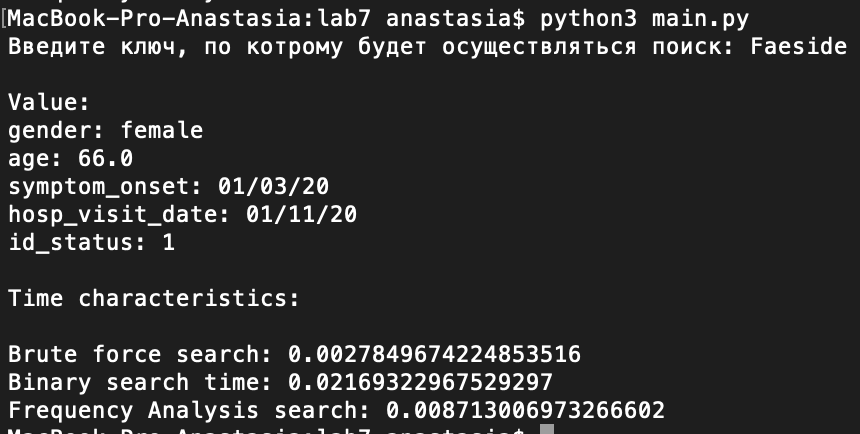
\includegraphics[scale=0.7]{pics/Best.png}
		
			Рис 4.1: Результат работы программы в лучшем случае
\end{center}

Результат свидетельствует о том, что в лучшем случае наиболее выигрышным по времени является алгоритм поиска полным перебором, так как искомый ключ найдется за 1 итерацию цикла поиска ключа в словаре.

На рис. 4.2 приведен графики зависимостей времени работы алгоритмов от размерности матрицы смежности.


\subsection{Худший случай}

Худшим случаем считается ситуация, когда искомый ключ располагается в конце словаря. На тестовой выборке данных person.csv последним элементом является пациент с именем Kantrius, который будет ключом в словаре. На рис. 4.2 представлен результат работы программы.

\begin{center}
		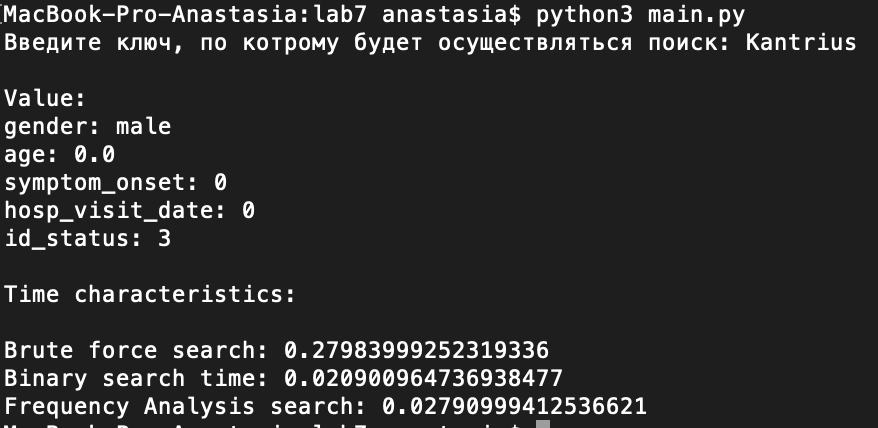
\includegraphics[scale=0.7]{pics/Worst.png}
		
			Рис 4.2: Результат работы программы в худшем случае
\end{center}

Результат свидетельствует о том, что в худшем случае наиболее выигрышным по времени является алгоритм двоичного поиска, так как искомый ключ найдется за N итераций цикла поиска ключа в словаре и при таком условии алгоритм полного перебора и частичного анализа работают медленнее за счет большого количества проходов цикла.

\subsection{Произвольная позиция в словаре}

На тестовой выборке данных person.csv произвольным элементом был взят пациент с именем Jonis, который будет ключом в словаре. На рис. 4.3 представлен результат работы программы.

\begin{center}
		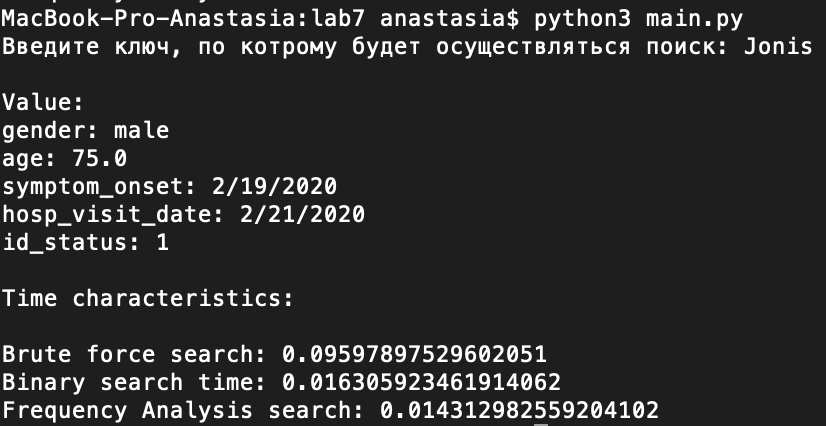
\includegraphics[scale=0.7]{pics/Random}
		
			Рис 4.3: Результат работы в случае, когда ключ находится в произвольном месте словаря
\end{center}

Результат свидетельствует о том, что в случае произвольной позиции ключа в словаре алгоритм поиска частичным анализом работает быстрее всего.

\subsection{Ключ не найден}

Был взят ключ, значения которого нет в тестовой выборке данных person.csv: Nastya. На рис. 4.4 представлен результат работы программы.

\begin{center}
		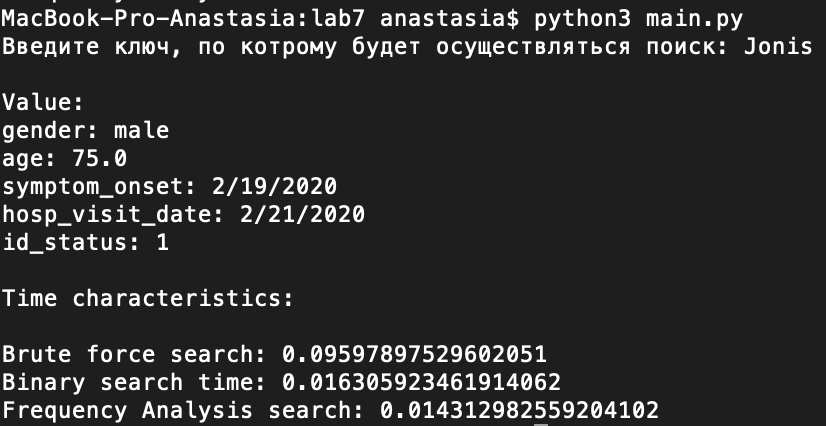
\includegraphics[scale=0.7]{pics/Random}
		
			Рис 4.4: Результат работы в случае, когда искомого ключа нет в словаре
\end{center}

Результат свидетельствует о том, что в случае, когда искомого ключа нет в словаре, алгоритм поиска частичным анализом работает быстрее всего.


\section{Вывод}

В результате сравнения алгоритма полного перебора, алгоритма двоичного поиска и алгоритма поиска частичным анализом было установлено, что в большинстве случаев алгоритм поиска полным перебором работает медленнее остальных, за исключением случая, когда искомый ключ находится в начале словаря. В худшем случае, когда ключ находится в конце словаря, по времени выигрышным оказывается алгоритм двоичного поиска. В остальных случаях выигрывает алгоритм поиска частичным анализом.

\chapter*{Заключение}
\addcontentsline{toc}{chapter}{Заключение}

В ходе лабораторной работы был изучен поиск значения по ключу в словаре с помощью алгоритмов поиска полным перебором, двоичного поиска в упорядоченном словаре и частичного анализа.

В рамках выполнения работы решены следующие задачи:

\begin{itemize}
\item изучен алгоритм поиска в словаре полным перебором;
\item изучен алгоритм двоичного поиска в упорядоченном словаре;
\item изучен алгоритм частичного анализа для поиска в словаре;
\item программно реализованы описанные выше алгоритмы;
\item проведен сравнительный анализ скорости работы реализованных алгоритмов.
\end{itemize}

%\bibliography{books}

\addcontentsline{toc}{chapter}{Список литературы}
\begin{thebibliography}{3}
	\bibitem{Vs}
	Visual Studio [Электронный ресурс], режим доступа:https://visualstudio.microsoft.com/ru/ (дата обращения: 01.10.2020)
	\bibitem{Python}
	Python [Электронный ресурс], режим доступа:https://www.python.org (дата обращения: 24.12.2020)
	 \bibitem{AntAlg}
	Муравьиные алгоритмы [Электронный ресурс], режим доступа:http://www.machinelearning.ru/wiki/index.php?title=Муравьиные\_алгоритмы (дата обращения: 20.12.2020)
	 \bibitem{AssocArray}
	NIST’s Dictionary of Algorithms and Data Structures: Associative Array [Электронный ресурс], режим доступа:https://xlinux.nist.gov/dads/HTML/assocarray.html (дата обращения: 21.12.2020)
	 \bibitem{Perl}
	The Perl Programming Language [Электронный ресурс], режим доступа:https://www.perl.org (дата обращения: 24.12.2020)
	\bibitem{Php}
	Руководство по PHP [Электронный ресурс], режим доступа:https://www.php.net/manual/ru/index.php (дата обращения: 24.12.2020)
	\bibitem{Ruby}
	Язык программирования Ruby [Электронный ресурс], режим доступа:https://www.ruby-lang.org/ru/ (дата обращения: 24.12.2020)
	\bibitem{JS}
	JavaScript [Электронный ресурс], режим доступа:https://developer.mozilla.org/ru/docs/Web/JavaScript (дата обращения: 24.12.2020)
	
	
	
\end{thebibliography}

\end{document}